<!-- Generated by pkgdown: do not edit by hand -->
<!DOCTYPE html>
<html lang="en">
  <head>
  <meta charset="utf-8">
<meta http-equiv="X-UA-Compatible" content="IE=edge">
<meta name="viewport" content="width=device-width, initial-scale=1.0">

<title>IBMPopSim description • IBMPopSim</title>


<!-- jquery -->
<script src="https://cdnjs.cloudflare.com/ajax/libs/jquery/3.4.1/jquery.min.js" integrity="sha256-CSXorXvZcTkaix6Yvo6HppcZGetbYMGWSFlBw8HfCJo=" crossorigin="anonymous"></script>
<!-- Bootstrap -->
<link href="https://cdnjs.cloudflare.com/ajax/libs/bootswatch/3.4.0/cosmo/bootstrap.min.css" rel="stylesheet" crossorigin="anonymous" />


<script src="https://cdnjs.cloudflare.com/ajax/libs/twitter-bootstrap/3.4.1/js/bootstrap.min.js" integrity="sha256-nuL8/2cJ5NDSSwnKD8VqreErSWHtnEP9E7AySL+1ev4=" crossorigin="anonymous"></script>

<!-- bootstrap-toc -->
<link rel="stylesheet" href="../bootstrap-toc.css">
<script src="../bootstrap-toc.js"></script>

<!-- Font Awesome icons -->
<link rel="stylesheet" href="https://cdnjs.cloudflare.com/ajax/libs/font-awesome/5.12.1/css/all.min.css" integrity="sha256-mmgLkCYLUQbXn0B1SRqzHar6dCnv9oZFPEC1g1cwlkk=" crossorigin="anonymous" />
<link rel="stylesheet" href="https://cdnjs.cloudflare.com/ajax/libs/font-awesome/5.12.1/css/v4-shims.min.css" integrity="sha256-wZjR52fzng1pJHwx4aV2AO3yyTOXrcDW7jBpJtTwVxw=" crossorigin="anonymous" />

<!-- clipboard.js -->
<script src="https://cdnjs.cloudflare.com/ajax/libs/clipboard.js/2.0.6/clipboard.min.js" integrity="sha256-inc5kl9MA1hkeYUt+EC3BhlIgyp/2jDIyBLS6k3UxPI=" crossorigin="anonymous"></script>

<!-- headroom.js -->
<script src="https://cdnjs.cloudflare.com/ajax/libs/headroom/0.11.0/headroom.min.js" integrity="sha256-AsUX4SJE1+yuDu5+mAVzJbuYNPHj/WroHuZ8Ir/CkE0=" crossorigin="anonymous"></script>
<script src="https://cdnjs.cloudflare.com/ajax/libs/headroom/0.11.0/jQuery.headroom.min.js" integrity="sha256-ZX/yNShbjqsohH1k95liqY9Gd8uOiE1S4vZc+9KQ1K4=" crossorigin="anonymous"></script>

<!-- pkgdown -->
<link href="../pkgdown.css" rel="stylesheet">
<script src="../pkgdown.js"></script>




<meta property="og:title" content="IBMPopSim description" />
<meta property="og:description" content="IBMPopSim" />




<!-- mathjax -->
<script src="https://cdnjs.cloudflare.com/ajax/libs/mathjax/2.7.5/MathJax.js" integrity="sha256-nvJJv9wWKEm88qvoQl9ekL2J+k/RWIsaSScxxlsrv8k=" crossorigin="anonymous"></script>
<script src="https://cdnjs.cloudflare.com/ajax/libs/mathjax/2.7.5/config/TeX-AMS-MML_HTMLorMML.js" integrity="sha256-84DKXVJXs0/F8OTMzX4UR909+jtl4G7SPypPavF+GfA=" crossorigin="anonymous"></script>

<!--[if lt IE 9]>
<script src="https://oss.maxcdn.com/html5shiv/3.7.3/html5shiv.min.js"></script>
<script src="https://oss.maxcdn.com/respond/1.4.2/respond.min.js"></script>
<![endif]-->



  </head>

  <body data-spy="scroll" data-target="#toc">
    <div class="container template-article">
      <header>
      <div class="navbar navbar-default navbar-fixed-top" role="navigation">
  <div class="container">
    <div class="navbar-header">
      <button type="button" class="navbar-toggle collapsed" data-toggle="collapse" data-target="#navbar" aria-expanded="false">
        <span class="sr-only">Toggle navigation</span>
        <span class="icon-bar"></span>
        <span class="icon-bar"></span>
        <span class="icon-bar"></span>
      </button>
      <span class="navbar-brand">
        <a class="navbar-link" href="../index.html">IBMPopSim</a>
        <span class="version label label-default" data-toggle="tooltip" data-placement="bottom" title="Released version">0.3.0</span>
      </span>
    </div>

    <div id="navbar" class="navbar-collapse collapse">
      <ul class="nav navbar-nav">
        <li>
  <a href="../index.html">
    <span class="fas fa fas fa-home fa-lg"></span>
     
  </a>
</li>
<li>
  <a href="../articles/IBMPopSim.html">Get started</a>
</li>
<li>
  <a href="../reference/index.html">Reference</a>
</li>
<li class="dropdown">
  <a href="#" class="dropdown-toggle" data-toggle="dropdown" role="button" aria-expanded="false">
    Articles
     
    <span class="caret"></span>
  </a>
  <ul class="dropdown-menu" role="menu">
    <li>
      <a href="../articles/IBMPopSim_human_pop.html">Human population</a>
    </li>
    <li>
      <a href="../articles/IBMPopSim_human_pop_IMD.html">Human population with swap</a>
    </li>
    <li>
      <a href="../articles/IBMPopSim_interaction.html">Population with genetically variable traits</a>
    </li>
  </ul>
</li>
      </ul>
      <ul class="nav navbar-nav navbar-right">
        <li>
  <a href="https://github.com/DaphneGiorgi/IBMPopSim/">
    <span class="fab fa fab fa-github fa-lg"></span>
     
  </a>
</li>
      </ul>
      
    </div><!--/.nav-collapse -->
  </div><!--/.container -->
</div><!--/.navbar -->

      

      </header>


<div class="row">
  <div class="col-md-9 contents">
    <div class="page-header toc-ignore">
      <h1 data-toc-skip>IBMPopSim description</h1>
                        <h4 class="author">Daphné Giorgi</h4>
                        <h4 class="author">Sarah Kaakaï</h4>
                        <h4 class="author">Vincent Lemaire</h4>
            
      
      <small class="dont-index">Source: <a href='https://github.com/DaphneGiorgi/IBMPopSim/blob/master/vignettes/IBMPopSim.Rmd'><code>vignettes/IBMPopSim.Rmd</code></a></small>
      <div class="hidden name"><code>IBMPopSim.Rmd</code></div>

    </div>

    
    
The IBMPopSim package is conceived to simulate the random evolution of structured population dynamics, called stochastic Individual Based Models (IBMs).

The package allows users to simulate the random evolution of a population in which individuals are characterized by their date of birth, a set of (discrete or continuous) attributes, and their potential date of death.\\
The population is modified due to different types of events defined by the user, and occurring at random dates. These events include the birth/arrival or death/exit of an individual in the population, an individual changing characteristics.
Once the events modifying the population have been defined, the last step before simulating the population evolution is to specify the so-called events intensities, describing the frequency at which the different types of events occur in the population.

\hypertarget{general-features-and-package-installation}{%
\section{General features and package installation}\label{general-features-and-package-installation}}

\hypertarget{brief-overview-of-individual-based-models-ibms}{%
\subsection{Brief overview of Individual-Based-Models (IBMs)}\label{brief-overview-of-individual-based-models-ibms}}

Stochastic Individual-Based-Models (IBMs) can be defined as a general class of population dynamics models, where different types of events can occur to individuals at random dates, depending on their characteristics and interactions with others.

The package IBMPopSim allows the efficient simulation of a wide class IBMs where individuals are marked by their age (or equivalently their date of birth) and a set of characteristics (gender, location, size, socioeconomic class\ldots). { champs d'application}

An IBM can always be summarized by the different types events that can occur to individuals and modify the population composition, and how frequently they happen. Let us start by recalling briefly these features before going into detailed on how they can be defined in IBMPopSim.

\hypertarget{eventsTh}{%
\subsubsection{Events type and associated kernel}\label{eventsTh}}

In IBMPopSim, the population can evolve according to six main types of events:

\begin{itemize}
\tightlist
\item
  \textbf{Birth event}: addition of an individual of age 0 to the population.
\item
  \textbf{Death event}: removal of an individual from the population.
\item
  \textbf{Entry event}: arrival of an individual in the population.
\item
  \textbf{Exit (emmigration) event}: exit from the population (other than death).
\item
  \textbf{Swap event}: an individual changes of characteristics.
\item
  \textbf{custom events}.
\end{itemize}

With each event type is associated an \textbf{event kernel}, describing how the population is modified following the occurrence of the event. For instance, if an individual \texttt{I} dies or exit a time \(t\), the individual is removed from the population.

For other types of events, the event kernel has to be specified. Indeed, if an new individual enters the population (entry event), the rule for choosing the age and characteristics of this new individual has to be defined.\\
For instance, the characteristics of a new individual in the population can be chosen uniformly in the space of all characteristics, or can depends on the distribution of his parents or those of the other individuals composing the population.

\hypertarget{Eventintensityth}{%
\subsubsection{Events intensity}\label{Eventintensityth}}

Once the different types or events and their action have been defined, it remains to define how frequently they can occur to define properly an IBM.

An event intensity a function

\begin{equation}
\lambda^e(I,t) = f(I,t,\dots)
(\#eq:intensity)
\end{equation}

describing the frequency at which an event \(e\) can occur to \emph{an individual} \texttt{I} in the population. Informally, given an history of the population \((\mathcal{F}_t)\),

\begin{equation}
\mathbb{P}(\text{event } e \text{ occurring to I during } ]t,t+dt] | \mathcal{F}_t) = \lambda^e(I,t).
\end{equation}

The intensity function \(\lambda^e\) can depend on:

\begin{itemize}
\tightlist
\item
  The individual's age and characteristics,
\item
  The time t,
\item
  Interactions with other individuals,
\item
  Other model parameters.
\end{itemize}

When the intensity \(\lambda^e\) does not depends on the other individuals living in the population (there are no interactions for this specific event), the intensity function is said to be in the class of \textbf{individual} intensity functions. This is case for instance when the death intensity of individuals only depend on their age and characteristics.\\
Otherwise, the intensity function is said to be the class of \textbf{interaction} functions. In this package, we mainly focus on ``quadratic interactions", that is of intensity functions of the form

\begin{equation}
\lambda^e(I,t) = \sum_{J \in pop} U(I,J,t),
  (\#eq:interaction)
\end{equation}

where the interaction function \(U(I,J,t)\) represent the interaction between two individuals \(I\) and \(J\) at time \(t\). See for instance the vignette {\ldots{}} for examples of intensities with interactions.

Sometimes, the intensity refers to the frequency at which an event can occur in \emph{all the population}. This is the case for instance when individuals enter the population at a constant rate \(C^e\) (intensity of class \texttt{poisson}), or at a rate only depending on time \((\Lambda^e_t)\) (intensity of class \texttt{inhomogeneous\_poisson}). In this case, the intensity \(\Lambda^e_t\) is informally defined as

\begin{equation}
\mathbb{P}(\text{event } e \text{ occurring to in the population during } ]t,t+dt] | \mathcal{F}_t) = \Lambda^e_t.
\end{equation}

\hypertarget{installation-and-quick-model-creation-and-simulation}{%
\subsection{Installation and quick model creation and simulation}\label{installation-and-quick-model-creation-and-simulation}}

\hypertarget{installation}{%
\subsubsection{Installation}\label{installation}}

\begin{Shaded}
\begin{Highlighting}[]
\KeywordTok{install.packages}\NormalTok{(}\StringTok{"IBMPopSim"}\NormalTok{)}

\KeywordTok{library}\NormalTok{(IBMPopSim)}
\end{Highlighting}
\end{Shaded}

\hypertarget{quick-model-creation-and-simulation}{%
\subsubsection{Quick model creation and simulation}\label{quick-model-creation-and-simulation}}

Before going into details on the different steps for defining an IBM in IBMPopSim, let us first go quickly through an example of model creation and simulation.\\
In order to define a model, the user must specify three building blocks:

\begin{itemize}
\tightlist
\item
  An initial population (see Section @ref(population)),
\item
  The model parameters (see Section @ref(params)),
\item
  The different events (see Section @ref(events)).
\end{itemize}

The model can then be created from these three blocks.

\begin{enumerate}
\def\labelenumi{\arabic{enumi}.}
\tightlist
\item
  We take here an initial population, stored in a dataframe, composed of 100 000 individuals marked by their gender (encoded by a Boolean characteristic):
\end{enumerate}

\begin{Shaded}
\begin{Highlighting}[]
\NormalTok{population\_df \textless{}{-}}\StringTok{ }\NormalTok{EW\_pop\_}\DecValTok{14}\OperatorTok{$}\NormalTok{sample}
\end{Highlighting}
\end{Shaded}

\begin{enumerate}
\def\labelenumi{\arabic{enumi}.}
\setcounter{enumi}{1}
\tightlist
\item
  The second step is to define the model parameters' list:
\end{enumerate}

\begin{Shaded}
\begin{Highlighting}[]
\NormalTok{params \textless{}{-}}\StringTok{ }\KeywordTok{list}\NormalTok{(}\StringTok{"alpha"}\NormalTok{ =}\StringTok{  }\FloatTok{0.008}\NormalTok{, }\StringTok{"beta"}\NormalTok{ =}\FloatTok{0.02}\NormalTok{, }\StringTok{"p\_male"}\NormalTok{=}\StringTok{ }\FloatTok{0.51}\NormalTok{,}
               \StringTok{"birth\_rate"}\NormalTok{ =}\StringTok{ }\KeywordTok{stepfun}\NormalTok{(}\KeywordTok{c}\NormalTok{(}\DecValTok{15}\NormalTok{,}\DecValTok{40}\NormalTok{),}\KeywordTok{c}\NormalTok{(}\DecValTok{0}\NormalTok{,}\FloatTok{0.05}\NormalTok{,}\DecValTok{0}\NormalTok{)))}
\end{Highlighting}
\end{Shaded}

\begin{enumerate}
\def\labelenumi{\arabic{enumi}.}
\setcounter{enumi}{2}
\tightlist
\item
  The last step is to defined the events that can occur in the population, here birth and death events:
\end{enumerate}

\begin{Shaded}
\begin{Highlighting}[]
\NormalTok{death\_event \textless{}{-}}\StringTok{ }\KeywordTok{mk\_event\_individual}\NormalTok{(}\DataTypeTok{type =} \StringTok{"death"}\NormalTok{,}
                  \DataTypeTok{intensity\_code =} \StringTok{" result = alpha*exp(beta*age(I, t));"}\NormalTok{)}

\NormalTok{birth\_event \textless{}{-}}\StringTok{ }\KeywordTok{mk\_event\_individual}\NormalTok{( }\DataTypeTok{type =} \StringTok{"birth"}\NormalTok{, }
                  \DataTypeTok{intensity\_code =} \StringTok{"result=birth\_rate(age(I,t));"}\NormalTok{,}
                  \DataTypeTok{kernel\_code =} \StringTok{"newI.male = CUnif(0, 1) \textless{} p\_male;"}\NormalTok{)}
\end{Highlighting}
\end{Shaded}

\begin{enumerate}
\def\labelenumi{\arabic{enumi}.}
\setcounter{enumi}{3}
\tightlist
\item
  Finally, the model is created by calling the function \texttt{mk\_model}
\end{enumerate}

\begin{Shaded}
\begin{Highlighting}[]
\NormalTok{model \textless{}{-}}\StringTok{ }\KeywordTok{mk\_model}\NormalTok{(}\DataTypeTok{characteristics =} \KeywordTok{get\_characteristics}\NormalTok{(population\_df),}
                  \DataTypeTok{events =} \KeywordTok{list}\NormalTok{(death\_event, birth\_event),}
                  \DataTypeTok{parameters =}\NormalTok{ params)}
\end{Highlighting}
\end{Shaded}

\begin{enumerate}
\def\labelenumi{\arabic{enumi}.}
\setcounter{enumi}{4}
\tightlist
\item
  In order to simulate a random trajectory of the population until a given time \texttt{T} bounds on the events intensities have to be specified:
\end{enumerate}

\begin{Shaded}
\begin{Highlighting}[]
\NormalTok{a\_max \textless{}{-}}\StringTok{ }\DecValTok{115}
\NormalTok{events\_bounds =}\StringTok{ }\KeywordTok{c}\NormalTok{( }\StringTok{"death"}\NormalTok{ =}\StringTok{ }\NormalTok{params}\OperatorTok{$}\NormalTok{alpha}\OperatorTok{*}\KeywordTok{exp}\NormalTok{(params}\OperatorTok{$}\NormalTok{beta}\OperatorTok{*}\NormalTok{a\_max),}
                   \StringTok{"birth"}\NormalTok{ =}\StringTok{ }\KeywordTok{max}\NormalTok{(params}\OperatorTok{$}\NormalTok{birth\_rate))}
\end{Highlighting}
\end{Shaded}

Then, the function \texttt{popsim} can be called:

\begin{Shaded}
\begin{Highlighting}[]
\NormalTok{sim\_out \textless{}{-}}\StringTok{ }\KeywordTok{popsim}\NormalTok{(model, population\_df, events\_bounds, params,}
                  \DataTypeTok{age\_max =}\NormalTok{ a\_max, }\DataTypeTok{time =} \DecValTok{30}\NormalTok{)}
\end{Highlighting}
\end{Shaded}

\begin{verbatim}
## Simulation on  [0, 30]
\end{verbatim}

\begin{enumerate}
\def\labelenumi{\arabic{enumi}.}
\setcounter{enumi}{5}
\tightlist
\item
  The dataframe \texttt{pop\_out\$population} contains the information (date of birth, date of death, gender) on individuals who lived in the population over the period \([0,30]\). Functions of the package allows to provide aggregated information on the population.
\end{enumerate}

\begin{Shaded}
\begin{Highlighting}[]
\NormalTok{pop\_out \textless{}{-}}\StringTok{ }\NormalTok{sim\_out}\OperatorTok{$}\NormalTok{population}
\NormalTok{female\_pop \textless{}{-}}\StringTok{ }\NormalTok{pop\_out[pop\_out}\OperatorTok{$}\NormalTok{male}\OperatorTok{==}\OtherTok{FALSE}\NormalTok{,]}
\KeywordTok{age\_pyramid}\NormalTok{(female\_pop, }\DataTypeTok{ages =} \DecValTok{85}\OperatorTok{:}\DecValTok{90}\NormalTok{, }\DataTypeTok{time =} \DecValTok{30}\NormalTok{)}
\end{Highlighting}
\end{Shaded}

\begin{verbatim}
##       age  male value
## 1 85 - 86 FALSE   222
## 2 86 - 87 FALSE   249
## 3 87 - 88 FALSE   211
## 4 88 - 89 FALSE   187
## 5 89 - 90 FALSE   202
\end{verbatim}

\begin{Shaded}
\begin{Highlighting}[]
\NormalTok{Dxt \textless{}{-}}\StringTok{ }\KeywordTok{death\_table}\NormalTok{(female\_pop, }\DataTypeTok{ages =} \DecValTok{85}\OperatorTok{:}\DecValTok{90}\NormalTok{,}\DataTypeTok{times =} \DecValTok{20}\OperatorTok{:}\DecValTok{30}\NormalTok{)}
\NormalTok{Ext \textless{}{-}}\StringTok{ }\KeywordTok{exposure\_table}\NormalTok{(female\_pop, }\DataTypeTok{ages =} \DecValTok{85}\OperatorTok{:}\DecValTok{90}\NormalTok{,}\DataTypeTok{times =} \DecValTok{20}\OperatorTok{:}\DecValTok{30}\NormalTok{)}
\end{Highlighting}
\end{Shaded}

\begin{enumerate}
\def\labelenumi{\arabic{enumi}.}
\setcounter{enumi}{7}
\tightlist
\item
  Parameters of the model can be changed without recompiling the model.
\end{enumerate}

\begin{Shaded}
\begin{Highlighting}[]
\NormalTok{params}\OperatorTok{$}\NormalTok{beta  \textless{}{-}}\StringTok{ }\FloatTok{0.01}

\CommentTok{\# Update death event bound:}
\NormalTok{events\_bounds[}\StringTok{"death"}\NormalTok{]\textless{}{-}}\StringTok{ }\NormalTok{params}\OperatorTok{$}\NormalTok{alpha}\OperatorTok{*}\KeywordTok{exp}\NormalTok{(params}\OperatorTok{$}\NormalTok{beta}\OperatorTok{*}\NormalTok{a\_max)}

\NormalTok{pop\_out \textless{}{-}}\StringTok{ }\KeywordTok{popsim}\NormalTok{(model, population\_df, events\_bounds, params,}
                  \DataTypeTok{age\_max =}\NormalTok{ a\_max, }\DataTypeTok{time =} \DecValTok{30}\NormalTok{)}
\end{Highlighting}
\end{Shaded}

\hypertarget{package-description}{%
\section{Package description}\label{package-description}}

The first step to define a model in IBMPopSim is to define the population structure.

\hypertarget{population}{%
\subsection{Population}\label{population}}

\hypertarget{initial-population}{%
\subsubsection{Initial population}\label{initial-population}}

A population is a dataframe in which each row corresponds to an individual, and
which has at least two columns:

\begin{itemize}
\tightlist
\item
  A column \texttt{birth} containing the birth dates of individuals in the population.
\item
  A column \texttt{death} containing the birth dates of individuals in the population ( \texttt{NA} for alive individuals).
\end{itemize}

The dataframe can contain more than two columns if individuals are described by additional characteristics such as gender, size, spatial location\ldots{}

\begin{Shaded}
\begin{Highlighting}[]
\KeywordTok{head}\NormalTok{(population\_df)}
\end{Highlighting}
\end{Shaded}

\begin{verbatim}
##       birth death  male
## 1 -106.9055    NA FALSE
## 2 -106.8303    NA FALSE
## 3 -104.5097    NA  TRUE
## 4 -104.2218    NA FALSE
## 5 -103.5225    NA FALSE
## 6 -103.3644    NA FALSE
\end{verbatim}

In the example above, individuals are described by their birth and death dates, as well a Boolean characteristics called \texttt{male}. For instance, the first individual is a female whose age at \(t_0=0\) is \(t_0 - (-106.9055) = 106.9055\).

We draw the attention to the fact that some characteristics names are forbidden, or are reserved to specific cases. The reserved words include:

\begin{itemize}
\tightlist
\item
  \texttt{male}: can only be used for a Boolean characteristics, usually referring to the individuals' sex/gender.
\item
  \texttt{id}: can only be used in order to defined the individuals unique identifier (see Section @ref(simulationswap)).
\item
  \texttt{time} : forbidden as characteristics or variable name.\\
\item
  C++ reserved words: forbidden as characteristics or variable name. Note that \texttt{char}
  is a reserved word. See \href{https://en.cppreference.com/w/cpp/keyword}{here} for a comprehensive list of C++ reserved words.
\end{itemize}

Attention: I, J, pop, newI, t, k

\hypertarget{individuals}{%
\subsubsection{Individuals}\label{individuals}}

During the model creation, a population of individuals is created from the initial population dataframe. The C++ class \texttt{individual} contains several useful functions, whose context of use is detailed in the following. For instance,

\begin{itemize}
\tightlist
\item
  \texttt{age(I,t)} returns the age of an individual \texttt{I} at time \texttt{t}.
\item
  \texttt{newI.set\_age(a,t)} sets the birth date \(t-a\) of a new individual called \texttt{newI}, of age \texttt{a} at time \texttt{t}.
\end{itemize}

If \texttt{Chi} is the name of a characteristic, then \texttt{I.Chi} returns the value of the characteristic \texttt{Chi} for the individual \texttt{I}. For instance, in the previous example \texttt{I.male} would equal to \texttt{TRUE} if \texttt{I} is a male of \texttt{FALSE} if \texttt{I} is a female.

\hypertarget{params}{%
\subsection{Model parameters}\label{params}}

A list of model parameters can be defined to simplify the events creation. These parameters can be of various types, summarized in the following table:

\begin{longtable}[]{@{}ll@{}}
\caption{(\#tab:unnamed-chunk-11)Parameters}\tabularnewline
\toprule
Types of parameters & Parameters\tabularnewline
\midrule
\endfirsthead
\toprule
Types of parameters & Parameters\tabularnewline
\midrule
\endhead
\texttt{R} objects & Numeric, logical, character\tabularnewline
\texttt{Armadillo} objects & Vector (\texttt{arma::vec}), matrix (numeric) (\texttt{arma::mat})\tabularnewline
List of IBMPopSim functions & \texttt{gompertz}, \texttt{stepfun}, \texttt{piecewise\_x}, \texttt{piecewise\_xy}, \texttt{weibull}\tabularnewline
\bottomrule
\end{longtable}

For example,

\begin{Shaded}
\begin{Highlighting}[]
\NormalTok{params \textless{}{-}}\StringTok{ }\KeywordTok{list}\NormalTok{(}\StringTok{"coeff"}\NormalTok{ =}\StringTok{ }\FloatTok{1.1}\NormalTok{,}
                \StringTok{"death\_function"}\NormalTok{ =}\StringTok{ }\KeywordTok{gompertz}\NormalTok{(}\FloatTok{0.1}\NormalTok{,}\FloatTok{0.005}\NormalTok{))}
\end{Highlighting}
\end{Shaded}

creates a numeric parameter \texttt{coeff} and a Gompertz function \texttt{death\_function} which can be used when creating the events of the model.

\textbf{IBMPopSim functions} are classes of functions predefined in the package to simplify models creation. For instance, \texttt{gompertz(a,b)} returns the function \(g(x) = a \exp(bx)\)
and \texttt{stepfun} is the usual R function for the creation of step functions. Another example is \texttt{piecewise\_xy} which allow the creation of age and time functions. See Section @ref(IBMfunctions) for a description of all IBM functions, and Section @ref(armadillo) for more details of Armadillo objects.

\hypertarget{events}{%
\subsection{Events creations}\label{events}}

The last and most important step of the model creation is the events creation. The call to the function creating an event is of form,

\texttt{mk\_event\_CLASS(type\ =\ "TYPE",\ name\ ="NAME",\ kernel\_code\ =\ "KERNEL\_CODE",\ ...)}

where \texttt{CLASS} is replaced by the class of the event intensity, \texttt{type} is the event type and \texttt{kernel\_code} the event kernel.

The other arguments depend on the intensity class. Tables @ref(tab:evtype) and @ref(tab:evclass) summarize the different intensity classes and types of events introduced in Section @ref(eventsTh).

\begin{longtable}[]{@{}ll@{}}
\caption{(\#tab:evtype)Event types}\tabularnewline
\toprule
Event type & \texttt{Type}\tabularnewline
\midrule
\endfirsthead
\toprule
Event type & \texttt{Type}\tabularnewline
\midrule
\endhead
Birth & \texttt{birth}\tabularnewline
Entry & \texttt{entry}\tabularnewline
Death & \texttt{death}\tabularnewline
Exit & \texttt{exit}\tabularnewline
Swap & \texttt{swap}\tabularnewline
Custom & \texttt{custom}\tabularnewline
\bottomrule
\end{longtable}

\begin{longtable}[]{@{}ll@{}}
\caption{(\#tab:evclass)Intensity classes}\tabularnewline
\toprule
Intensity class & \texttt{Class}\tabularnewline
\midrule
\endfirsthead
\toprule
Intensity class & \texttt{Class}\tabularnewline
\midrule
\endhead
Poisson & \texttt{poisson}\tabularnewline
Inhomogeneous Poisson & \texttt{inohomogeneous\_poisson}\tabularnewline
Individual & \texttt{individual}\tabularnewline
Interaction & \texttt{interaction}\tabularnewline
\bottomrule
\end{longtable}

Tables @ref(tab:evtype) ou @ref(evtype).

The intensity function and kernel of an event are defined through arguments of the function \texttt{mk\_event\_CLASS}. These arguments are strings composed of few lines of code defining an event frequency and its action of the event on individuals. Since the model is compiled using Rcpp, the code should be written in C++. However, thanks to the model parameters and functions/variables of the package, even the non-experienced C++ user can define a model quite easily. Several examples are given in the several vignettes of this package, and basic C++ tools are presented in Section @ref(essentials).

The optional argument \texttt{name} gives a name to the event. If not specified, the name of the event is its type, for instance \texttt{death}. However, a name must be specified if the model is composed of several events with the same name.

\hypertarget{event-type-and-kernel-code}{%
\subsubsection{Event type and kernel code}\label{event-type-and-kernel-code}}

The argument \texttt{kernel\_code} is \texttt{NULL} by default and doesn't have to be specified for death and exit events. For those types of events, the event kernel is automatically generated during the model creation. For instance, if the user defines a \textbf{death event}, the C++ code generated is

\texttt{pop.kill(k,\ t);}

which removes the individual number \texttt{k} from the population \texttt{pop} if he dies. No kernel has to be specified by the user.

If an \textbf{exit events} is defined, a characteristic \texttt{out} is automatically added to individuals in the population. When an individual \texttt{I} exit the population,\texttt{I.out} is set \texttt{TRUE} and his exit time is recorded as a ``death'' date.

For a \textbf{birth event}, the default generated event kernel is that an individual \texttt{I} gives birth to a new individual \texttt{newI} of age 0 at the current time \texttt{t}, which has the same characteristics than his parent \texttt{I}. If no kernel is specified, the default generated C++ code for a birth event is:

\begin{verbatim}
individual newI = I; 
newI.birth_date = t;  
pop.add(newI); 
\end{verbatim}

The user can modify the birth kernel, by specify the argument `\texttt{kernel\_code} of \texttt{mk\_event\_CLASS}. In this case, the generated code is

\begin{verbatim}
individual newI = I;   
newI.birth_date = t;  
_KERNEL_CODE_
pop.add(newI);
\end{verbatim}

where \texttt{\_KERNEL\_CODE\_} is replaced by the content of the \texttt{kernel\_code} argument. For instance, in a population where individuals are characterized by their gender, the kernel code

\begin{Shaded}
\begin{Highlighting}[]
\NormalTok{birth\_kernel\_code \textless{}{-}}\StringTok{ "newI.male = (CUnif(0, 1) \textless{} p\_male);"}
\end{Highlighting}
\end{Shaded}

creates new individuals which are males with probability \texttt{p\_male}, or females otherwise. Here, \texttt{p\_male} should be included in the parameters of the model.

When an \textbf{entry events} occurs the individual entering the population is not of age \(0\). In this case, the user must specify the \texttt{kernel\_code} argument indicating how the age and characteristics of the new individual are chosen. For instance, with

\begin{Shaded}
\begin{Highlighting}[]
\NormalTok{entry\_kernel\_code \textless{}{-}}\StringTok{ "double a = CUnif(20,40); }
\StringTok{                      newI.set\_age(a,t); }
\StringTok{                      newI.male = (CUnif(0, 1) \textless{} p\_male);}
\StringTok{                      newI.immigrant =TRUE;"}
\end{Highlighting}
\end{Shaded}

individuals who enter the population have age \texttt{a} taken uniformly in \([20,40]\). In this example, the characteristic \texttt{immigrant} has been added to the population to distinguish individuals who entered the population from individuals ``born in the population''.

The available variables for the birth and entry events C++ kernel codes are:

\begin{longtable}[]{@{}ll@{}}
\caption{(\#tab:varBirth)C++ variables available for birth and entry events kernel code}\tabularnewline
\toprule
Variable & Description\tabularnewline
\midrule
\endfirsthead
\toprule
Variable & Description\tabularnewline
\midrule
\endhead
\texttt{I} & Current individual\tabularnewline
\texttt{t} & Current time\tabularnewline
\texttt{pop} & Current population (vector)\tabularnewline
\texttt{newI} & New individual. By default \texttt{newI\ =\ I} with \texttt{newI.birth\ =\ t}\tabularnewline
Model parameters & Depends on the model\tabularnewline
\bottomrule
\end{longtable}

Finally, the C++ kernel code for a \textbf{swap event} is only specified by the \texttt{kernel\_code} argument of \texttt{mk\_event\_CLASS} which must specify how the new characteristics of the individual are chosen. The kernel code can depend on the following variables:

\begin{longtable}[]{@{}ll@{}}
\caption{(\#tab:varSwap)C++ variables available for swap events kernel code}\tabularnewline
\toprule
Variable & Description\tabularnewline
\midrule
\endfirsthead
\toprule
Variable & Description\tabularnewline
\midrule
\endhead
\texttt{I} & Current individual\tabularnewline
\texttt{t} & Current time\tabularnewline
\texttt{pop} & Current population (vector)\tabularnewline
Model parameters & Depends on the model\tabularnewline
\bottomrule
\end{longtable}

We can now describe the different intensity classes.

\hypertarget{event-creation-with-individual-intensity}{%
\subsubsection{Event creation with individual intensity}\label{event-creation-with-individual-intensity}}

As explained in @ref(Eventintensityth), events with intensities in the class \texttt{individual} are intensity functions which depend only the individual age and characteristics and on time.\\
They are created using the function

\begin{verbatim}
mk_event_individual(type = "TYPE", name ="name" 
                    intensity_code = "INTENSITY",   
                    kernel_code = "KERNEL_CODE"),
\end{verbatim}

The \texttt{intensity\_code} argument contains few lines C++ code describing the intensity function. The available variables for the intensity code are given in Table @ref(tab:varInd) :

\begin{longtable}[]{@{}ll@{}}
\caption{(\#tab:varInd)C++ variables available for individual intensities}\tabularnewline
\toprule
Variable & Description\tabularnewline
\midrule
\endfirsthead
\toprule
Variable & Description\tabularnewline
\midrule
\endhead
\texttt{I} & Current individual\tabularnewline
\texttt{t} & Current time\tabularnewline
Model parameters & Depends on the model\tabularnewline
\bottomrule
\end{longtable}

The intensity value has to be stored in a variable called \texttt{result}. For instance, the intensity code

\begin{Shaded}
\begin{Highlighting}[]
\NormalTok{death\_intensity\textless{}{-}}\StringTok{ " if (I.male)}
\StringTok{                      result = alpha\_1*exp(beta\_1*age(I, t));}
\StringTok{                    else}
\StringTok{                      result = alpha\_2*exp(beta\_2*age(I,t));"}
\end{Highlighting}
\end{Shaded}

corresponds to a death intensity equal to \(d_1(a) = \alpha_1 \exp(\beta_1 a)\) for males and \(d_2(a) = \alpha_2 \exp(\beta_2 a)\) for females. In this case, the intensity function depends on the individuals' age, gender, and on the model parameters \(\alpha = (\alpha_1, \alpha_2)\) and \(\beta = (\beta_1, \beta_2)\).

The code

\begin{Shaded}
\begin{Highlighting}[]
\NormalTok{time\_dep\_function \textless{}{-}}\StringTok{ }\KeywordTok{piecewise\_xy}\NormalTok{(}\KeywordTok{c}\NormalTok{(}\DecValTok{5}\NormalTok{),}
                                  \KeywordTok{list}\NormalTok{(}\KeywordTok{gompertz}\NormalTok{(}\FloatTok{0.1}\NormalTok{,}\FloatTok{0.005}\NormalTok{), }
                                       \KeywordTok{gompertz}\NormalTok{(}\FloatTok{0.08}\NormalTok{,}\FloatTok{0.005}\NormalTok{)))}
\KeywordTok{time\_dep\_function}\NormalTok{(}\DecValTok{0}\NormalTok{,}\DecValTok{65}\NormalTok{) }\CommentTok{\# death intensity at time 0 and age 65.}
\end{Highlighting}
\end{Shaded}

\begin{verbatim}
## [1] 0.1384031
\end{verbatim}

\begin{Shaded}
\begin{Highlighting}[]
\NormalTok{params \textless{}{-}}\StringTok{ }\KeywordTok{list}\NormalTok{(}\StringTok{"death\_function"}\NormalTok{=}\StringTok{ }\NormalTok{time\_dep\_function)}

\NormalTok{time\_dep\_intensity\textless{}{-}}\StringTok{ "result=death\_function(t,age(I,t));"}
\end{Highlighting}
\end{Shaded}

creates a death intensity depending on a age and time, equal to

\begin{equation*}
d(t,a) = 0.1\exp(0.005a) 1_{\{0\leq t <5\}} + 0.08\exp(0.005a) 1_{\{5\leq t\}} 
\end{equation*}

\hypertarget{event-creation-with-interaction-intensity}{%
\subsubsection{Event creation with interaction intensity}\label{event-creation-with-interaction-intensity}}

Events with intensities in the class \texttt{interaction} are events which occur to an individual at a frequency which is the result of interactions with other members of the population (see @ref(Eventintensityth)), and which can be written as

\begin{equation*}
\lambda^e(I,t) = \sum_{J \in pop} U(I,J,t),
  (\#eq:interaction)
\end{equation*}

where \(U(I,J,t)\) is the intensity of the interaction between individual \(I\) and \(J\).

An event with intensity in the class \texttt{interaction} is created by calling the function

\begin{verbatim}
mk_event_interaction(type = "TYPE",  
    interaction_code = "INTERACTION_CODE",  
    interaction_type="random",
    kernel_code = "KERNEL_CODE").
\end{verbatim}

The \texttt{intensity\_code} argument contains few lines of C++ code describing
the interaction function \(U\). The available variables for the intensity code are:

\begin{table}

\caption{(\#tab:varInt)C++ variables available for interaction code}
\centering
\begin{tabular}[t]{l|l}
\hline
Variable & Description\\
\hline
`I` & Current individual\\
\hline
`J` & Another individual in the population\\
\hline
`t` & Current time\\
\hline
Model parameters & Depends on the model\\
\hline
\end{tabular}
\end{table}

Here is example of interaction code:

\begin{Shaded}
\begin{Highlighting}[]
\NormalTok{death\_interaction\_code\textless{}{-}}\StringTok{ " result = max(J.size {-}I.size,0);"}
\end{Highlighting}
\end{Shaded}

In the example above, the death intensity of an individual \texttt{I} is the result of competition between individuals, depending on a characteristic named \texttt{size}. If \texttt{I} meets randomly an individual \texttt{J} of size bigger than \texttt{I.size}, he can die at the intensity \texttt{J.size-I.size}. The bigger is \texttt{I.size}, the lower is the death intensity of individual \texttt{I}.

The argument \texttt{interaction\_type}, set by default at \texttt{random}, is an algorithm choice for simulating the model.\\
When \texttt{interaction\_type=full}, the intensity of an individual is computed making the sum over all the individuals in the population of the interactions with the given individual. In IBMPopSim, we introduced a ``randomized'' algorithm, in which the intensity of an individual is computed by picking randomly another individual in the population and computing its interaction function with the given individual. In most cases, the \texttt{random} algorithm is much faster than the \texttt{full} algorithm.

Note that events with individual intensities are also much faster to simulate since they only require to observe \emph{one} individual to be computed.

\hypertarget{poisson-and-inhomogeneous-poisson-events-creation}{%
\subsubsection{Poisson and Inhomogeneous Poisson events creation}\label{poisson-and-inhomogeneous-poisson-events-creation}}

When a event occur in the population with an intensity which does not depend on the population, the event intensity is of (inhomogeneous) Poisson class. When the event intensity is simply a constant, the class is called Poisson in reference to Poisson processes intensities. Such events are created with the function

\begin{verbatim}
mk_event_poisson(type="TYPE",   
                 intensity="CONSTANT",   
                 kernel_code = "KERNEL_CODE")
\end{verbatim}

If the parameters \texttt{lambda} has been defined in the list of model parameters, then

\begin{Shaded}
\begin{Highlighting}[]
\KeywordTok{mk\_event\_poisson}\NormalTok{(}\DataTypeTok{type =} \StringTok{"entry"}\NormalTok{, }\DataTypeTok{intensity =} \StringTok{"lambda"}\NormalTok{, }
                 \DataTypeTok{kernel\_code =}\StringTok{"double a\_I= CNorm(20,2); }
\StringTok{                               newI.set\_age(a\_I,t);"}\NormalTok{)}
\end{Highlighting}
\end{Shaded}

creates an event of type Entry, where individuals enter the population at a constant intensity \texttt{lambda}. When an individual \texttt{newI} enters the population at time \texttt{t}, his age is chosen as a normally distributed random variable, with mean 20 and variance 4, using the function \texttt{CNorm()} ({ see doc }).
When the intensity depends on time (but not on the population), the event can be created similarly by using the function

\begin{verbatim}
mk_event_inhomogeneous_poisson(type= "TYPE",   
                               intensity_code = "INTENSITY",   
                               kernel_code = "KERNEL_CODE")
\end{verbatim}

For instance,

\begin{Shaded}
\begin{Highlighting}[]
\KeywordTok{mk\_event\_inhomogeneous\_poisson}\NormalTok{(}\DataTypeTok{type =} \StringTok{"entry"}\NormalTok{,    }
                               \DataTypeTok{intensity =} \StringTok{"result = lambda*cos(t);"}\NormalTok{, }
                               \DataTypeTok{kernel\_code =}\StringTok{" double a\_I= CNorm(20,2); }
\StringTok{                                             newI.set\_age(a\_I,t);"}\NormalTok{)}
\end{Highlighting}
\end{Shaded}

creates the same event than before, but now individuals enter the population at the rate \(\lambda \cos(t)\) depending on the current time \texttt{t}.

\hypertarget{Modelcreation}{%
\subsection{Model creation}\label{Modelcreation}}

Finally, the IBM model is created using the function \texttt{mk\_model}. The model is composed of:

\begin{itemize}
\tightlist
\item
  The characteristics names and types, which can be obtained from a population dataframe with the function \texttt{get\_characteristics},
\item
  The events list,
\item
  The model parameters.
\end{itemize}

\begin{Shaded}
\begin{Highlighting}[]
\NormalTok{model \textless{}{-}}\StringTok{ }\KeywordTok{mk\_model}\NormalTok{(}\DataTypeTok{characteristics =} \KeywordTok{get\_characteristics}\NormalTok{(population\_df),}
                  \DataTypeTok{event =}\NormalTok{ events\_list,}
                  \DataTypeTok{parameters =}\NormalTok{ model\_params)}
\end{Highlighting}
\end{Shaded}

During this step which can take a few seconds, the model is created and compiled using the Rcpp package.
One of the advantages of the model structure in IBMPopSim is that only the model only depends on the population characteristics' and parameters names and types, rather than their values.

This means that once the model has been created, various simulations can be done with various initial populations and different parameters values. Thus, only one model has to be created to simulation a class of IBMs with varying parameters (see Section @ref(Simulation1) for an example).

Here is an example of model with a gender characteristic and two events (birth and death):

\begin{Shaded}
\begin{Highlighting}[]
\NormalTok{params \textless{}{-}}\StringTok{ }\KeywordTok{list}\NormalTok{(}\StringTok{"p\_male"}\NormalTok{=}\StringTok{ }\FloatTok{0.51}\NormalTok{, }
               \StringTok{"birth\_rate"}\NormalTok{ =}\StringTok{ }\KeywordTok{stepfun}\NormalTok{(}\KeywordTok{c}\NormalTok{(}\DecValTok{15}\NormalTok{,}\DecValTok{40}\NormalTok{),}\KeywordTok{c}\NormalTok{(}\DecValTok{0}\NormalTok{,}\FloatTok{0.05}\NormalTok{,}\DecValTok{0}\NormalTok{)),}\StringTok{"death\_rate"}\NormalTok{=}\KeywordTok{gompertz}\NormalTok{(}\FloatTok{0.008}\NormalTok{,}\FloatTok{0.02}\NormalTok{))}


\NormalTok{death\_event \textless{}{-}}\StringTok{ }\KeywordTok{mk\_event\_individual}\NormalTok{(}\DataTypeTok{type =} \StringTok{"death"}\NormalTok{, }\DataTypeTok{name=} \StringTok{"my\_death\_event"}\NormalTok{,}
                  \DataTypeTok{intensity\_code =} \StringTok{"result = death\_rate(age(I,t));"}\NormalTok{)}

\NormalTok{birth\_event \textless{}{-}}\StringTok{ }\KeywordTok{mk\_event\_individual}\NormalTok{( }\DataTypeTok{type =} \StringTok{"birth"}\NormalTok{, }
                  \DataTypeTok{intensity\_code =} \StringTok{" if (I.male)}
\StringTok{                                        result = 0; }
\StringTok{                                     else }
\StringTok{                                        result=birth\_rate(age(I,t));"}\NormalTok{,}
                  \DataTypeTok{kernel\_code =} \StringTok{"newI.male = CUnif(0, 1) \textless{} p\_male;"}\NormalTok{)}


\NormalTok{model \textless{}{-}}\StringTok{ }\KeywordTok{mk\_model}\NormalTok{(}\DataTypeTok{characteristics =} \KeywordTok{get\_characteristics}\NormalTok{(population\_df),}
                  \DataTypeTok{events =} \KeywordTok{list}\NormalTok{(death\_event,birth\_event),}
                  \DataTypeTok{parameters =}\NormalTok{ params)}

\KeywordTok{summary}\NormalTok{(model)}
\end{Highlighting}
\end{Shaded}

\begin{verbatim}
## Events:
## #1: individual event of type death
## #2: individual event of type birth
## --------------------------------------- 
## Individual description:
## names:  birth death male 
## R types:  double double logical 
## C types:  double double bool
## --------------------------------------- 
## R parameters available in C++ code:
## names:  p_male birth_rate death_rate 
## R types:  double closure closure 
## C types:  double function_x function_x
\end{verbatim}

\hypertarget{simulation}{%
\subsection{Simulation and outputs}\label{simulation}}

Once the model has been created, the random evolution of the population can be simulated over a period of time \([0,T]\) by calling the function

\begin{verbatim}
popsim(model,population, events_bounds, parameters,age_max,time,...)
\end{verbatim}

Where:

\begin{itemize}
\tightlist
\item
  \texttt{model} is the model created in the previous step,
\item
  \texttt{population} is a population dataframe representing the initial population,
\item
  \texttt{parameters} is the list of parameters value,
\item
  \texttt{age\_max} is the maximum age of individuals in the population (set by default to \texttt{Inf}),
\item
  \texttt{time} is the final simulation time \(T\) or a vector of times (see @ref(simulation\_swap)),
\item
  \texttt{events\_bounds} is a named vector of \textbf{bounds} for the intensity or interaction function of each event.
\end{itemize}

\hypertarget{algorithm-and-events-bounds}{%
\subsubsection{Algorithm and events bounds}\label{algorithm-and-events-bounds}}

The IBM simulation algorithm is based on an acceptance-rejection method for simulating random times, called thinning ({donner ref}). The main idea of the algorithm is to simulate candidate event times with \emph{constant} intensity \(\bar \lambda\) (which is simply an exponential variable with parameter \(\lambda\)), which \emph{dominates} the true event intensity \(\lambda^e(I,t)\) for all individuals \(I\):

\begin{equation}
\lambda^e(I,t) \leq \bar{\lambda}, \quad \forall I \in \text{pop}, \; t \in [0,T].
\end{equation}

Starting from time \(t\), once a candidate event time \(t + \tau^e\) has been proposed for a given event \(e\) and individual \(I\), it remains to accept or reject the candidate event with probability \(\frac{\lambda^e(I,t+\tau^e)}{\bar{\lambda}}\). If the candidate event is accepted, then the event \(e\) occurs to the individual \(I\) at time \(t + \tau^e\). The thinning algorithm can be summarized as follow:

\textbf{Thinning algorithm}

\begin{enumerate}
\def\labelenumi{\arabic{enumi}.}
\tightlist
\item
  Draw a candidate time \(t+\tau^e\) for event \(e\), \(\tau^e \sim \mathcal E(\bar \lambda)\).
\item
  Draw a uniform variable \(\theta \sim \mathcal U([0,1])\).
\item
  \textbf{If} \(\theta \leq \dfrac{\lambda^e(I,t+\tau^e)}{\bar\lambda}\) \textbf{then}\\
  \(\qquad\) Apply event kernel to individual \(I\)\\
  \textbf{else}\\
  \(\qquad\) Do nothing and start again from \(t+\tau^e\).
\end{enumerate}

If the intensity is of class \texttt{interaction}, the intensity function \(\lambda^e\) is replaced by the interaction function \(U^e\), and \(\bar \lambda\) by a bound \(\bar U^e\) of \(U^e\).

Thus, before simulating a random path of the population evolution, the user has to specify bounds for the intensity function (resp. interaction kernel) of each event. Let us consider the model with a birth and death built in the previous section.

In the model, the birth intensity of an individual of age \(a\) is \(0\) if he is a male, and
\[ b(a) = 0.005  \mathbb{1}_{[15,40]},\]
if the individual is a female. Thus, the intensity bound for birth events is

\[\bar\lambda_b = \sup_{a\geq 0} \;  \text{birth\_rate}(a) = 0.05\]

Since the death intensity function is not bounded, the user will have to specify a maximum age \(a_{max}\) in \texttt{popsim}. Then, the bound for death events is

\[ \bar \lambda_d = 0.008\exp(0.02 a_{max}).\]

The events bounds are defined as a \emph{named} R vector, with components names corresponding to the events names.\\
In our example, the event of type death has been named \texttt{"my\_death\_event"}. No name has been specified for the event of type birth which thus has the default name \texttt{"birth"}. Then,

\begin{Shaded}
\begin{Highlighting}[]
\NormalTok{a\_max \textless{}{-}}\StringTok{ }\DecValTok{120} \CommentTok{\# maximum age}
\NormalTok{events\_bounds \textless{}{-}}\StringTok{ }\KeywordTok{c}\NormalTok{(}\StringTok{"my\_death\_event"}\NormalTok{ =}\StringTok{ }\FloatTok{0.008}\OperatorTok{*}\KeywordTok{exp}\NormalTok{(}\FloatTok{0.02}\OperatorTok{*}\NormalTok{a\_max),}
                  \StringTok{"birth"}\NormalTok{ =}\StringTok{ }\KeywordTok{max}\NormalTok{(params}\OperatorTok{$}\NormalTok{birth\_rate))}

\NormalTok{events\_bounds}
\end{Highlighting}
\end{Shaded}

\begin{verbatim}
## my_death_event          birth 
##     0.08818541     0.05000000
\end{verbatim}

{ Utilisation de max, renvoyer à la section C++. }

\hypertarget{Simulation1}{%
\subsubsection{Simulation without swap events}\label{Simulation1}}

Once the model and events bounds have been defined, a random trajectory of the population can be simulated by calling

\begin{Shaded}
\begin{Highlighting}[]
\NormalTok{sim\_out \textless{}{-}}\StringTok{ }\KeywordTok{popsim}\NormalTok{(model, population\_df, events\_bounds, params,}
                  \DataTypeTok{age\_max =}\NormalTok{ a\_max, }\DataTypeTok{time =} \DecValTok{30}\NormalTok{)}
\end{Highlighting}
\end{Shaded}

\begin{verbatim}
## Simulation on  [0, 30]
\end{verbatim}

\begin{Shaded}
\begin{Highlighting}[]
\CommentTok{\#str(sim\_out)}
\end{Highlighting}
\end{Shaded}

\texttt{sim\_out} is a list composed of

\begin{itemize}
\tightlist
\item
  A list \texttt{arguments} of the simulation inputs, including the initial population, parameters and event bounds.
\item
  A named numeric vector \texttt{logs} of variables related to the simulation algorithm.
\item
  The simulation output called \texttt{population}.
\end{itemize}

When there are no swap events (individuals don't change of characteristics), the evolution of the population over the period \([0,30]\) is recorded in a single dataframe \texttt{sim\_out\$population} containing the information of all individuals who lived in the population during the period.\\
Each line of \texttt{sim\_out\$population} contains the information of an individual who lived in the population over the period \([0,30]\). This includes individuals who were initially in \texttt{population\_df}, as well as individuals who were born or entered the population.

\begin{Shaded}
\begin{Highlighting}[]
\KeywordTok{str}\NormalTok{(sim\_out}\OperatorTok{$}\NormalTok{population)}
\end{Highlighting}
\end{Shaded}

\begin{verbatim}
## 'data.frame':    118275 obs. of  3 variables:
##  $ birth: num  -90 -89.9 -89.9 -89.9 -89.9 ...
##  $ death: num  NA NA NA NA NA NA NA NA NA NA ...
##  $ male : logi  FALSE FALSE FALSE FALSE FALSE FALSE ...
\end{verbatim}

Table @ref(tab:logs) describes the elements of the vector \texttt{sim\_out\$logs}containing information on simulation algorithm:

\begin{table}

\caption{(\#tab:logs)Logs parameters}
\centering
\begin{tabular}[t]{l|l}
\hline
Elements & Description\\
\hline
`proposed\_events` & Number of candidate event times proposed during the simulation\\
\hline
`effective\_events` & Number of events which occured during the simulation\\
\hline
`cleanall\_counter` & Number of population cleans\\
\hline
`duration\_main\_algorithm` & Simulation time\\
\hline
\end{tabular}
\end{table}

For instance, the acceptance rate in the toy model is

\begin{Shaded}
\begin{Highlighting}[]
\NormalTok{sim\_out}\OperatorTok{$}\NormalTok{logs[}\StringTok{\textquotesingle{}effective\_events\textquotesingle{}}\NormalTok{]}\OperatorTok{/}\NormalTok{sim\_out}\OperatorTok{$}\NormalTok{logs[}\StringTok{\textquotesingle{}proposed\_events\textquotesingle{}}\NormalTok{]}
\end{Highlighting}
\end{Shaded}

\begin{verbatim}
## effective_events 
##        0.2182352
\end{verbatim}

and the simulation time is

\begin{Shaded}
\begin{Highlighting}[]
\NormalTok{sim\_out}\OperatorTok{$}\NormalTok{logs[}\StringTok{\textquotesingle{}duration\_main\_algorithm\textquotesingle{}}\NormalTok{]}
\end{Highlighting}
\end{Shaded}

\begin{verbatim}
## duration_main_algorithm 
##                0.078262
\end{verbatim}

\textbf{Parameters modification and event removal}

As explained in Section @ref(Modelcreation) the structure of the compiled model allows the parameters' values to be changed without recompiling the model. For instance, the parameter of the Gompertz death function can be modified to study the impact of an increase in mortality.\\
Before running the simulation, the events bounds should be updated accordingly accordingly.

\begin{Shaded}
\begin{Highlighting}[]
\NormalTok{params}\OperatorTok{$}\NormalTok{death\_rate \textless{}{-}}\StringTok{ }\KeywordTok{gompertz}\NormalTok{(}\FloatTok{0.01}\NormalTok{,}\FloatTok{0.02}\NormalTok{)}

\NormalTok{events\_bounds[}\StringTok{"my\_death\_event"}\NormalTok{] \textless{}{-}}\StringTok{ }\FloatTok{0.01}\OperatorTok{*}\KeywordTok{exp}\NormalTok{(}\FloatTok{0.02}\OperatorTok{*}\NormalTok{a\_max) }\CommentTok{\# Death event bound update}

\NormalTok{new\_sim\_out  \textless{}{-}}\StringTok{ }\KeywordTok{popsim}\NormalTok{(model, population\_df, events\_bounds, params,}
                  \DataTypeTok{age\_max =}\NormalTok{ a\_max, }\DataTypeTok{time =} \DecValTok{30}\NormalTok{) }\CommentTok{\# Population simulation }
\end{Highlighting}
\end{Shaded}

An event can also be remove by setting the event bound to 0:

\begin{Shaded}
\begin{Highlighting}[]
\NormalTok{sim\_out\_no\_birth \textless{}{-}}\StringTok{ }\KeywordTok{popsim}\NormalTok{(model, population\_df, }\DataTypeTok{events\_bounds =} \KeywordTok{c}\NormalTok{(}\StringTok{"birth"}\NormalTok{=}\DecValTok{0}\NormalTok{, }\StringTok{"my\_death\_event"}\NormalTok{=}\StringTok{ }\FloatTok{0.01}\OperatorTok{*}\KeywordTok{exp}\NormalTok{(}\FloatTok{0.02}\OperatorTok{*}\NormalTok{a\_max)),}
\NormalTok{                                params, }\DataTypeTok{age\_max =}\NormalTok{ a\_max, }\DataTypeTok{time =} \DecValTok{30}\NormalTok{) }\CommentTok{\# Simulation without birth events}
\end{Highlighting}
\end{Shaded}

\begin{verbatim}
## [1] "event birth is deactivated"
## Simulation on  [0, 30]
\end{verbatim}

\textbf{Outputs}

The R dataframe format for the output of the simulation allows all data manipulation functionalities of tidyverse or data.table packages to be used for analyzing the population. IBMPopSim also provides base functions to study the simulation outputs.

For instance, the population age pyramid can computed at a give time (resp. at multiple dates) with the function \texttt{age\_pyramid} (resp. \texttt{age\_pyramids}). We refer to the other vignettes for more details on age pyramids computation and visualization.

\begin{Shaded}
\begin{Highlighting}[]
\NormalTok{pop\_out \textless{}{-}}\StringTok{ }\NormalTok{sim\_out}\OperatorTok{$}\NormalTok{population}

\CommentTok{\# Population age{-}pyramid at time 30:}
\NormalTok{pyr \textless{}{-}}\StringTok{ }\KeywordTok{age\_pyramid}\NormalTok{(pop\_out, }\DataTypeTok{ages =} \DecValTok{0}\OperatorTok{:}\NormalTok{a\_max, }\DataTypeTok{time =} \DecValTok{30}\NormalTok{) }
\KeywordTok{plot\_pyramid}\NormalTok{(pyr)}
\end{Highlighting}
\end{Shaded}

\begin{center}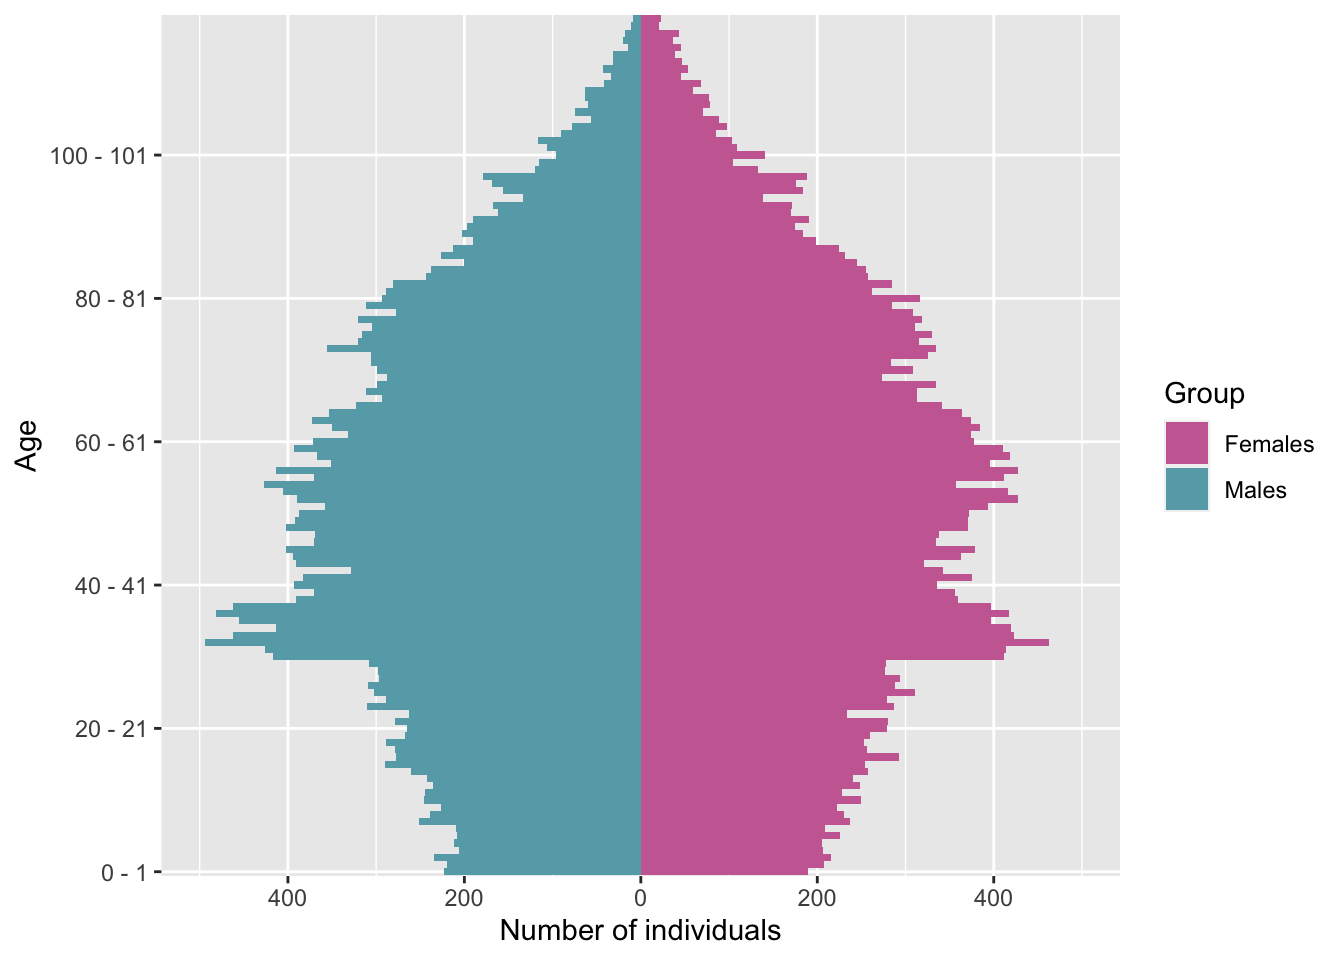
\includegraphics{/Users/lemaire/Travail/Codes/IBMPopSim/docs/articles/IBMPopSim_files/figure-latex/unnamed-chunk-30-1} \end{center}

Mortality tables with compatibles with packages such as StMoMo can also be computed by with the functions \texttt{death\_table} and \texttt{exposure\_table}.

\begin{Shaded}
\begin{Highlighting}[]
\NormalTok{female\_pop \textless{}{-}}\StringTok{ }\NormalTok{pop\_out[pop\_out}\OperatorTok{$}\NormalTok{male}\OperatorTok{==}\OtherTok{FALSE}\NormalTok{, ]}
\NormalTok{Dxt \textless{}{-}}\StringTok{ }\KeywordTok{death\_table}\NormalTok{(female\_pop, }\DataTypeTok{ages =} \DecValTok{85}\OperatorTok{:}\DecValTok{90}\NormalTok{,}\DataTypeTok{times =} \DecValTok{20}\OperatorTok{:}\DecValTok{30}\NormalTok{) }\CommentTok{\# Death table (death age is age at death)}
\NormalTok{Ext \textless{}{-}}\StringTok{ }\KeywordTok{exposure\_table}\NormalTok{(female\_pop, }\DataTypeTok{ages =} \DecValTok{85}\OperatorTok{:}\DecValTok{90}\NormalTok{,}\DataTypeTok{times =} \DecValTok{20}\OperatorTok{:}\DecValTok{30}\NormalTok{) }\CommentTok{\# Exact computation of central Exposure{-}to{-}risk}
\end{Highlighting}
\end{Shaded}

\textbf{Simple multithreading}

If there are \textbf{no interactions} between individuals, i.e.~if there are no events with intensity of class \texttt{interaction}, then the simulation can be parallelized easily by setting the optional parameter \texttt{multithreading} (\texttt{FALSE} by default) to \texttt{TRUE}:

\begin{Shaded}
\begin{Highlighting}[]
\NormalTok{sim\_out \textless{}{-}}\StringTok{ }\KeywordTok{popsim}\NormalTok{(model, population\_df, events\_bounds, params,}
                  \DataTypeTok{age\_max =}\NormalTok{ a\_max, }\DataTypeTok{time =} \DecValTok{30}\NormalTok{, }\DataTypeTok{multithreading =} \OtherTok{TRUE}\NormalTok{)}
\end{Highlighting}
\end{Shaded}

\begin{verbatim}
## duration_main_algorithm 
##                0.053349
\end{verbatim}

By default, the number of threads is the number of concurrent threads supported by the available hardware implementation.\\
The number of thread can be set manually with the optional argument \texttt{num\_threads} of \texttt{popsim}.

\hypertarget{simulationswap}{%
\subsection{Simulation with swap events}\label{simulationswap}}

When there are swap events (individuals can change of characteristics), the dates of swap events and the individual changed characteristics following each swap event should be recorded for each individual in the population, which is a memory intensive and computationally costly process.\\
To maintain efficient simulations in the presence of swap events, we propose the following solution:

\begin{enumerate}
\def\labelenumi{\arabic{enumi}.}
\tightlist
\item
  Use a vector of dates \((t_0,\dots, t_n)\) in the argument \texttt{time} of \texttt{popsim}. Then \texttt{popsim} returns in the object \texttt{population} a list of \(n\) population dataframes representing the population at time \(t_1,\dots t_n\), simulated from the initial time \(t_0\).\\
  For \(i=1\dots n\), the \(i\)th dataframe describes individuals who lived in the population during the period \([t_0,t_i]\), with their characteristics at time \(t_i\).
\end{enumerate}

In the following toy model, a population 100 thousand individuals (or particles) is generated, all born at time 0 and divided into two subgroups. Individuals can swap from subgroup 1 (resp. 2) to subgroup 2 (resp. 1) at rate 0.1 (resp. 0.3).

\begin{Shaded}
\begin{Highlighting}[]
\NormalTok{population\_df \textless{}{-}}\StringTok{ }\KeywordTok{data.frame}\NormalTok{(}\StringTok{"birth"}\NormalTok{=}\StringTok{ }\KeywordTok{rep}\NormalTok{(}\DecValTok{0}\NormalTok{,}\FloatTok{1e5}\NormalTok{),}\StringTok{"death"}\NormalTok{=}\KeywordTok{rep}\NormalTok{(}\OtherTok{NA}\NormalTok{,}\FloatTok{1e5}\NormalTok{), }
                         \StringTok{"sub\_grp"}\NormalTok{ =}\StringTok{ }\KeywordTok{sample}\NormalTok{(}\DecValTok{1}\OperatorTok{:}\DecValTok{2}\NormalTok{, }\FloatTok{1e5}\NormalTok{, }\DataTypeTok{replace =} \OtherTok{TRUE}\NormalTok{))}

\NormalTok{rates \textless{}{-}}\StringTok{ }\KeywordTok{list}\NormalTok{( }\DataTypeTok{k12 =} \FloatTok{0.1}\NormalTok{, }\DataTypeTok{k21=}\FloatTok{0.3}\NormalTok{)}
\CommentTok{\#Only swap events occur in the population}
\NormalTok{swap\_event \textless{}{-}}\StringTok{ }\KeywordTok{mk\_event\_individual}\NormalTok{( }\DataTypeTok{type =} \StringTok{"swap"}\NormalTok{, }
                  \DataTypeTok{intensity\_code =} \StringTok{"if (I.sub\_grp==1) result= k12 ; }
\StringTok{                                    else result= k21;"}\NormalTok{,}
                  \DataTypeTok{kernel\_code =} \StringTok{"I.sub\_grp = 3 {-} I.sub\_grp;"}\NormalTok{)}

\NormalTok{model\_swap \textless{}{-}}\StringTok{ }\KeywordTok{mk\_model}\NormalTok{(}\DataTypeTok{characteristics =}\KeywordTok{get\_characteristics}\NormalTok{(population\_df), }\DataTypeTok{events =} \KeywordTok{list}\NormalTok{(swap\_event),}\DataTypeTok{parameters =}\NormalTok{ rates)}
\end{Highlighting}
\end{Shaded}

Then, the population is simulated from \(t_0=0\) to \(t_n =20\), and \texttt{popsim} returns a list of 20 dataframes composed of the population at times \(t=1\dots 20\).

\begin{Shaded}
\begin{Highlighting}[]
\NormalTok{time\_vec \textless{}{-}}\StringTok{ }\DecValTok{1}\OperatorTok{:}\DecValTok{20}

\NormalTok{sim\_out \textless{}{-}}\KeywordTok{popsim}\NormalTok{(}\DataTypeTok{model =}\NormalTok{ model\_swap, }\DataTypeTok{population =}\NormalTok{ population\_df, }\DataTypeTok{events\_bounds =} \KeywordTok{c}\NormalTok{(}\StringTok{"swap"}\NormalTok{=}\KeywordTok{max}\NormalTok{(}\KeywordTok{unlist}\NormalTok{(rates))), }
                 \DataTypeTok{parameters =}\NormalTok{  rates, }\DataTypeTok{time =} \KeywordTok{c}\NormalTok{(}\DecValTok{0}\NormalTok{,time\_vec), }\DataTypeTok{multithreading =} \OtherTok{TRUE}\NormalTok{)}
\end{Highlighting}
\end{Shaded}

The model is an ergodic two states continuous time Markov chain with stationary distribution \((p_1,p_2)=(0,75,0.25)\). The figure below illustrates the convergence of the probability to be in subgroup 1 to \(p_1\)

\begin{Shaded}
\begin{Highlighting}[]
\NormalTok{pop\_size \textless{}{-}}\StringTok{ }\KeywordTok{nrow}\NormalTok{(population\_df)}
\CommentTok{\# Mean number of individuals in subgroup 1 at each time:}
\NormalTok{p\_}\DecValTok{1}\NormalTok{\_t \textless{}{-}}\StringTok{ }\KeywordTok{lapply}\NormalTok{(sim\_out}\OperatorTok{$}\NormalTok{population, }\ControlFlowTok{function}\NormalTok{(pop\_df)\{}
                      \KeywordTok{return}\NormalTok{(}\KeywordTok{nrow}\NormalTok{(}\KeywordTok{subset}\NormalTok{(pop\_df, sub\_grp}\OperatorTok{==}\DecValTok{1}\NormalTok{))}\OperatorTok{/}\NormalTok{pop\_size)}
\NormalTok{                \})}
\end{Highlighting}
\end{Shaded}

\begin{figure}

{\centering 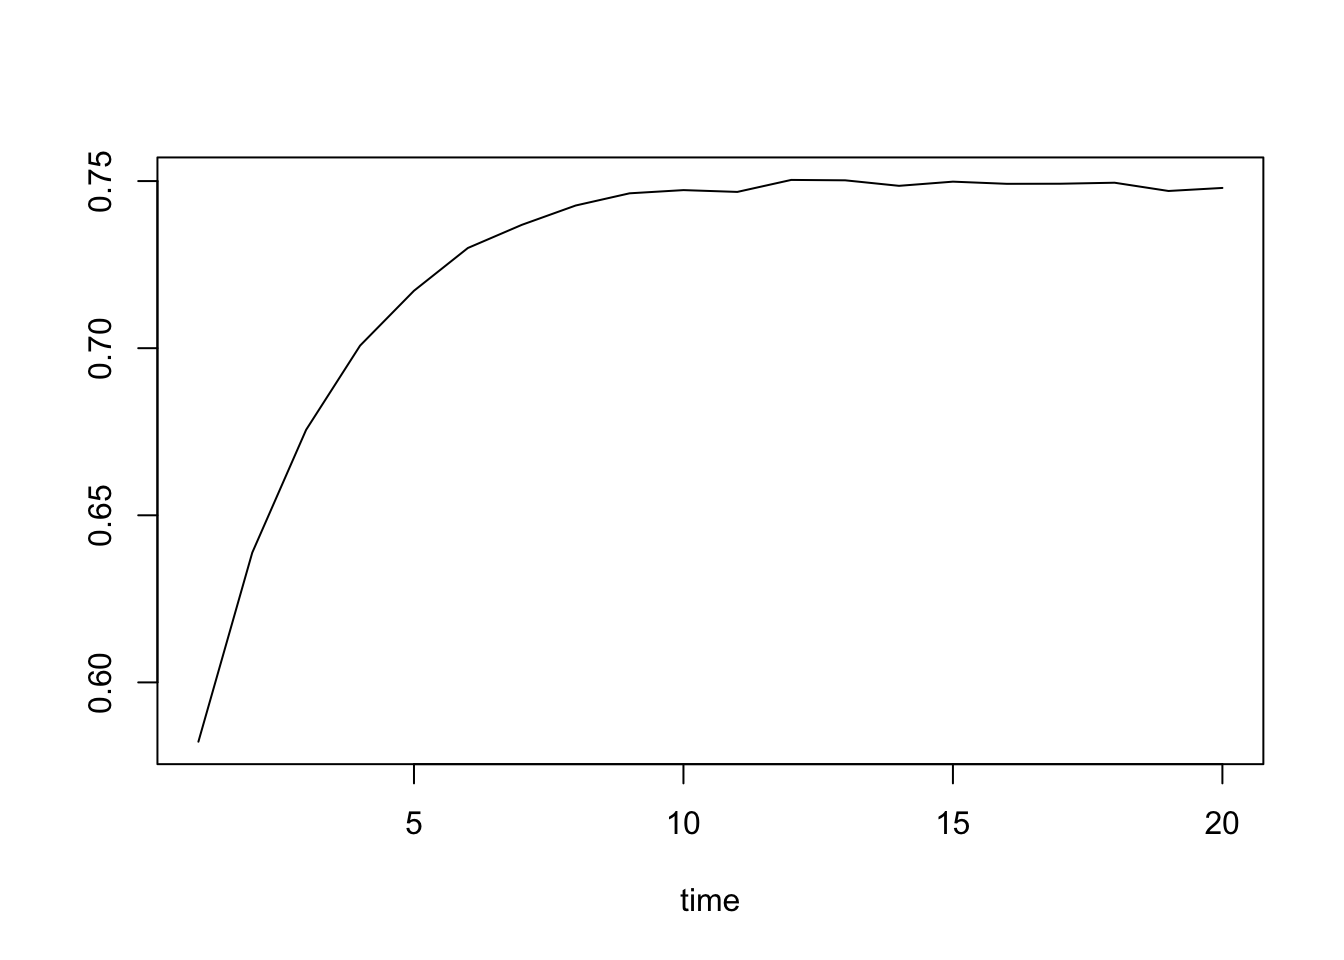
\includegraphics{/Users/lemaire/Travail/Codes/IBMPopSim/docs/articles/IBMPopSim_files/figure-latex/plot-1} 

}

\caption{Evolution of probability to be in subgroup 1}(\#fig:plot)
\end{figure}

This example shows that any continuous time Markov Chain with finite state space can be simulated in a few steps with IBMPopSim.

\begin{enumerate}
\def\labelenumi{\arabic{enumi}.}
\setcounter{enumi}{1}
\tightlist
\item
  {[}Optional{]} Activate the optional argument \texttt{with\_id} during the model creation step.
\end{enumerate}

It is possible to isolate the individuals' life course, by setting the optional argument \texttt{with\_id} of \texttt{mk\_model} to \texttt{TRUE}. In this case, a new characteristic called \texttt{id} is added to the population (if not already defined), identifying each individual with a unique integer.

\begin{Shaded}
\begin{Highlighting}[]
\NormalTok{model\_swap\_id \textless{}{-}}\StringTok{ }\KeywordTok{mk\_model}\NormalTok{(}\DataTypeTok{characteristics =}  \KeywordTok{get\_characteristics}\NormalTok{(population\_df), }\DataTypeTok{events =} \KeywordTok{list}\NormalTok{(swap\_event), }
                          \DataTypeTok{parameters =}\NormalTok{ rates, }\DataTypeTok{with\_id =} \OtherTok{TRUE}\NormalTok{)          }
\end{Highlighting}
\end{Shaded}

\begin{verbatim}
## [1] "add 'id' as individual attributes"
\end{verbatim}

\begin{Shaded}
\begin{Highlighting}[]
\NormalTok{sim\_out\_id \textless{}{-}}\KeywordTok{popsim}\NormalTok{(}\DataTypeTok{model =}\NormalTok{ model\_swap\_id, }
                    \DataTypeTok{population =}\NormalTok{ population\_df, }
                    \DataTypeTok{parameters =}\NormalTok{ rates, }
                    \DataTypeTok{events\_bounds =} \KeywordTok{c}\NormalTok{(}\StringTok{"swap"}\NormalTok{=}\FloatTok{0.3}\NormalTok{),}
                    \DataTypeTok{time =} \KeywordTok{seq}\NormalTok{(}\DecValTok{0}\NormalTok{,}\DecValTok{5}\NormalTok{, }\DataTypeTok{by=}\DecValTok{1}\NormalTok{), }
                    \DataTypeTok{multithreading =} \OtherTok{TRUE}\NormalTok{)}
\end{Highlighting}
\end{Shaded}

\begin{verbatim}
## [1] "Add 'id' attributes to the population."
## Simulation on  [0, 1]  [1, 2]  [2, 3]  [3, 4]  [4, 5]
\end{verbatim}

\begin{Shaded}
\begin{Highlighting}[]
\KeywordTok{head}\NormalTok{(sim\_out\_id}\OperatorTok{$}\NormalTok{population[[}\DecValTok{1}\NormalTok{]])}
\end{Highlighting}
\end{Shaded}

\begin{verbatim}
##   id birth death sub_grp
## 1  1     0    NA       1
## 2  5     0    NA       2
## 3  9     0    NA       1
## 4 13     0    NA       2
## 5 17     0    NA       2
## 6 21     0    NA       2
\end{verbatim}

These dataframes can be merged into a single dataframe summarizing the life course of each individual, by calling the function \texttt{merge\_pop\_withid}.

\begin{Shaded}
\begin{Highlighting}[]
\NormalTok{pop\_list \textless{}{-}}\StringTok{ }\NormalTok{sim\_out\_id}\OperatorTok{$}\NormalTok{population}
\NormalTok{pop\_merge \textless{}{-}}\StringTok{ }\KeywordTok{merge\_pop\_withid}\NormalTok{(pop\_list)}
\KeywordTok{head}\NormalTok{(pop\_merge)}
\end{Highlighting}
\end{Shaded}

\begin{verbatim}
##   id birth death sub_grp_1 sub_grp_2 sub_grp_3 sub_grp_4 sub_grp_5
## 1  1     0    NA         1         1         1         2         2
## 2  5     0    NA         2         2         2         1         1
## 3  9     0    NA         1         1         1         1         2
## 4 13     0    NA         2         2         2         2         2
## 5 17     0    NA         2         2         2         1         1
## 6 21     0    NA         2         2         1         1         2
\end{verbatim}

For instance, a transition from subgroup 1 to subgroup 2 is observed for the individual with \texttt{id} number 5, between time 2 and 3.

\hypertarget{essentials}{%
\section{C++ essentials}\label{essentials}}

The arguments \texttt{intensity\_code} and \texttt{kernel\_code} of the \texttt{mk\_event\_CLASS} functions must contain some C++ code given by the user. In this section we give the essential tools to write this little code.

\hypertarget{c-syntax}{%
\subsection{C++ syntax}\label{c-syntax}}

\begin{itemize}
\tightlist
\item
  Each statement must be ended by a semicolon.
\item
  Single-line comments start with two forward slashes \texttt{//}.
\item
  To create a variable, you must specify the type and assign it a value (type variable = value;). Here some examples:
\end{itemize}

\begin{verbatim}
int myNum = 5;               // Integer (whole number without decimals)
double myFloatNum = 5.99;    // Floating point number (with decimals)
char myLetter = 'D';         // Character
string myText = "Hello";     // String (text)
bool myBoolean = true;       // Boolean (true or false)
\end{verbatim}

\begin{itemize}
\tightlist
\item
  \texttt{bool} data type can take the values \texttt{true} (1) or \texttt{false} (0).
\item
  C++ supports the usual logical conditions from mathematics:

  \begin{itemize}
  \tightlist
  \item
    Less than: \texttt{a\ \textless{}\ b}
  \item
    Less than or equal to: \texttt{a\ \textless{}=\ b}
  \item
    Greater than: \texttt{a\ \textgreater{}\ b}
  \item
    Greater than or equal to: \texttt{a\ \textgreater{}=\ b}
  \item
    Equal to \texttt{a\ ==\ b}
  \item
    Not Equal to: \texttt{a\ !=\ b}
  \end{itemize}
\item
  Use the \texttt{if}, \texttt{else\ if}, \texttt{else} statements to specify a block of C++ code to be executed if one or more conditions are or not \texttt{true}.
\end{itemize}

\begin{verbatim}
if (condition1) {
  // block of code to be executed if condition1 is true
} else if (condition2) {
  // block of code to be executed if the condition1 is false and condition2 is true
} else {
  // block of code to be executed if the condition1 is false and condition2 is false
}
\end{verbatim}

\begin{itemize}
\tightlist
\item
  When you know exactly how many times you want to loop through a block of code, use the \texttt{for} loop.
\end{itemize}

\begin{verbatim}
for (statement 1; statement 2; statement 3) {
  // code block to be executed
}

//example
for (int i = 0; i < 5; i++) {
  cout << i << "\n";
}
\end{verbatim}

\begin{itemize}
\tightlist
\item
  The while loop loops through a block of code as long as a specified condition is true.
\end{itemize}

\begin{verbatim}
while (condition) {
  // code block to be executed
}
\end{verbatim}

\hypertarget{usual-numeric-functions}{%
\subsection{Usual numeric functions}\label{usual-numeric-functions}}

The most popular functions of the \texttt{\textless{}cmath\textgreater{}} library, which is included in the package, are listed in the table below. If the user wants to call some other functions of \texttt{cmath} not listed in the table, this is possible by adding the prefix \texttt{std::} to the name of the function.

\begin{longtable}[]{@{}lll@{}}
\toprule
Function name & Function call & Meaning\tabularnewline
\midrule
\endhead
max & max(a,b) & \(\max(a,b)\)\tabularnewline
min & min(a,b) & \(\min(a,b)\)\tabularnewline
log & log(x) & \(\log(x)=ln(x)\)\tabularnewline
exp & exp(x) & \(e^x\)\tabularnewline
sin & sin(x) & \(\sin(x)\)\tabularnewline
cos & cos(x) & \(\cos(x)\)\tabularnewline
pow & pow(x,a) & \(x^a\)\tabularnewline
sqrt & sqrt(x) & \(\sqrt(x)\)\tabularnewline
abs & abs(x) & \(|x|\)\tabularnewline
ceil & ceil(x) & \(\lceil x \rceil\)\tabularnewline
floor & floor(x) & \(\lfloor x \rfloor\)\tabularnewline
\bottomrule
\end{longtable}

\hypertarget{random}{%
\subsection{Random}\label{random}}

We use the following notations to describe the available C++ random distributions.

\begin{itemize}
\tightlist
\item
  \(\mathcal{U}(a,b)\) : uniform distribution with density function \(f(x) = \frac{1}{b-a}\) for \(a\leq x <b\)
\item
  \(\mathcal{E}(\lambda)\) : exponential distribution with density function \(\lambda e^{-\lambda x}\) for \(x\geq 0\)
\item
  \(\mathcal{N}(\mu,\sigma)\) : Gaussian distribution with density function \(\frac{1}{\sigma\sqrt{2\pi}}e^{-\frac 1 2 \left( \frac{x-\mu}{\sigma}\right)^2}\)
\item
  \(\mathcal{D_n}\) : discrete distribution with \(n\) possible values and with probabilities \(\{ p_0, p_1, \ldots, p_{n-1}\}\) such that \(\mathbb{P}(i|(p_0, \ldots, p_{n-1})) = p_i/\sum_{k=0}^{n-1}p_k\) \(\forall i=0, \ldots, n-1\)
\end{itemize}

In the table below we show how to call them, which means how to make independent realizations of these random variables, and we give the reference to the C++ corresponding function of the \href{http://www.cplusplus.com/reference/random/}{\texttt{\textless{}random\textgreater{}} library} hidden in this call.

\begin{longtable}[]{@{}llll@{}}
\toprule
\begin{minipage}[b]{0.22\columnwidth}\raggedright
Function name\strut
\end{minipage} & \begin{minipage}[b]{0.22\columnwidth}\raggedright
Function call\strut
\end{minipage} & \begin{minipage}[b]{0.22\columnwidth}\raggedright
Meaning\strut
\end{minipage} & \begin{minipage}[b]{0.22\columnwidth}\raggedright
\texttt{\textless{}random\textgreater{}} original function\strut
\end{minipage}\tabularnewline
\midrule
\endhead
\begin{minipage}[t]{0.22\columnwidth}\raggedright
CUnif\strut
\end{minipage} & \begin{minipage}[t]{0.22\columnwidth}\raggedright
CUnif(a=0,b=1)\strut
\end{minipage} & \begin{minipage}[t]{0.22\columnwidth}\raggedright
\(\mathcal{U}(a,b)\)\strut
\end{minipage} & \begin{minipage}[t]{0.22\columnwidth}\raggedright
\href{http://www.cplusplus.com/reference/random/uniform_real_distribution/}{\texttt{uniform\_real\_distribution\textless{}double\textgreater{}}}\strut
\end{minipage}\tabularnewline
\begin{minipage}[t]{0.22\columnwidth}\raggedright
CExp\strut
\end{minipage} & \begin{minipage}[t]{0.22\columnwidth}\raggedright
CExp(\(\lambda=1\))\strut
\end{minipage} & \begin{minipage}[t]{0.22\columnwidth}\raggedright
\(\mathcal{E}(\lambda)\)\strut
\end{minipage} & \begin{minipage}[t]{0.22\columnwidth}\raggedright
\href{http://www.cplusplus.com/reference/random/exponential_distribution/}{\texttt{exponential\_distribution\textless{}double\textgreater{}}}\strut
\end{minipage}\tabularnewline
\begin{minipage}[t]{0.22\columnwidth}\raggedright
CNorm\strut
\end{minipage} & \begin{minipage}[t]{0.22\columnwidth}\raggedright
CNorm(\(\mu=0\), \(\sigma=1\))\strut
\end{minipage} & \begin{minipage}[t]{0.22\columnwidth}\raggedright
\(\mathcal{N}(\mu,\sigma)\)\strut
\end{minipage} & \begin{minipage}[t]{0.22\columnwidth}\raggedright
\href{http://www.cplusplus.com/reference/random/normal_distribution/}{\texttt{normal\_distribution\textless{}double\textgreater{}}}\strut
\end{minipage}\tabularnewline
\begin{minipage}[t]{0.22\columnwidth}\raggedright
CDiscrete\strut
\end{minipage} & \begin{minipage}[t]{0.22\columnwidth}\raggedright
CDiscrete(p\_begin, p\_end)\strut
\end{minipage} & \begin{minipage}[t]{0.22\columnwidth}\raggedright
\(\mathcal{D_n}\)\strut
\end{minipage} & \begin{minipage}[t]{0.22\columnwidth}\raggedright
\href{http://www.cplusplus.com/reference/random/discrete_distribution/}{\texttt{discrete\_distribution\textless{}int\textgreater{}}}\strut
\end{minipage}\tabularnewline
\bottomrule
\end{longtable}

Here p\_begin and p\_end represent the iterators to the begin and to the end of an object which should be of size n, see the section ``Armadillo'' in order to see how to pass vectors or rows (columns) of a matrix to CDiscrete.

\hypertarget{armadillo}{%
\subsection{Armadillo}\label{armadillo}}

Two of the possible parameters types given in the argument \texttt{parameters} of the \texttt{mk\_model} function are R vectors (objects created with ``c(x\_1, \ldots,x\_n)'') and R matrices. These types are converted, using the \href{http://dirk.eddelbuettel.com/code/rcpp.armadillo.html}{RcppArmadillo library}, in C++ \href{http://arma.sourceforge.net/}{Armadillo} types, \texttt{arma::vec} and \texttt{arma::matrix} respectively.

Let v be a an object of type \texttt{arma::vec} and A be a an object of type \texttt{arma::matrix}. Here we show how to get the begin and the end iterators of these objects.

\begin{itemize}
\tightlist
\item
  v.begin(): iterator pointing to the begin of v
\item
  v.end(): iterator pointing to the end of v
\item
  A.begin\_row(i) : iterator pointing to the first element of row i
\item
  A.end\_row(i) : iterator pointing to the last element of row i
\item
  A.begin\_col(i) : iterator pointing to the first element of column i
\item
  A.end\_col(i) : iterator pointing to the last element of column i
\end{itemize}

\hypertarget{IBMfunctions}{%
\subsection{IBMPopSim functions}\label{IBMfunctions}}

{ TO DO }
  </div>

  <div class="col-md-3 hidden-xs hidden-sm" id="pkgdown-sidebar">

        <nav id="toc" data-toggle="toc">
      <h2 data-toc-skip>Contents</h2>
    </nav>
      </div>

</div>



      <footer>
      <div class="copyright">
  <p>Developed by Daphné Giorgi, Sarah Kakaai, Vincent Lemaire.</p>
</div>

<div class="pkgdown">
  <p>Site built with <a href="https://pkgdown.r-lib.org/">pkgdown</a> 1.5.1.</p>
</div>

      </footer>
   </div>

  


  </body>
</html>

